\chapter{Background}

% The following sections give an overview of the Reinforcement Learning framework
% and some of its variations, provide some information about games-based
% artificial intelligence environments, and review recent work done on Real-Time
% Strategy games.

\section{Reinforcement Learning}

Reinforcement Learning is centered around the idea that a good chunk of problems
in control theory and artificial intelligence can be viewed as sequential
decision-making processes \citep{Sutton:1998:IRL:551283}. In the typically used
formalisation we call \emph{agent} all the parts of the problem that contribute
to the execution of the decision-making process, and \emph{environment}
everything outside of the agent. Given a discrete-time setting, the full system
is commonly described in the following way: at every episode $t$ the agent
receives some observation $s_t \in S$ from the environment, executes an action
$a_t \in A$ derived from a policy $\pi : S \rightarrow A$, and receives a reward
$r_{t+1} \in \mathbb{R}$ together with a new observation. The objective of
reinforcement learning algorithms usually consist in maximising the reward
received in a certain time frame using the experience gained by acting within
the environment.

\subsection{Markov Decision Processes}

The decision-making process becomes quickly intractable if the agent has to deal
with the entirety of the experience at every step, therefore we need a way to to
approximate perceptual history without losing important information.

We define \emph{Markov Decision Process} (MDP) a task in which the observation
and reward at a particular time depend entirely on the immediately previous
observation-action pair (Equation \ref{eq:rl_mdp}).

\begin{equation}
Pr(s_{t+1}, r_{t+1} | s_1, a_1, ... , s_t, a_t) = Pr(s_{t+1}, r_{t+1} |
s_t, a_t)
\label{eq:rl_mdp}
\end{equation}

The observed state $s_t$ is called the \emph{Markov State} and is defined as the
state that summarises all gained experience up until time $t$. If during a
particular task all the observations received by the agents are Markov states,
then the problem is defined \emph{fully observable}, otherwise it's
\emph{partially observable}. Our work focuses on fully observable problems, but
we will take partial observability into account towards the final chapters to
discuss some of the properties of this set of decision tasks. Additionally we
assume our tasks to be \emph{episodic}, which means that they possess a finite
horizon with a number of reachable terminal states, and that the environment and
the agent have finite action and state spaces $A$ and $S$.

In general MDPs define a transition probability distribution $P_a(s, s')$
describing the probability that the process might move into a new state $s'$
from state $s$ taking action $a$ (Equation \ref{eq:rl_trans}), and a reward
function $R_a(s, s')$ that provides the expected reward for such transition
(Equation \ref{eq:rl_rew}).

\begin{equation}
P_a(s, s') = Pr(s' | s, a)
\label{eq:rl_trans}
\end{equation}

\begin{equation}
R_a(s, s') = \mathbb{E}[r|s, s', a]
\label{eq:rl_rew}
\end{equation}

At every step the action taken by the agent is selected by a policy $\pi(s, a) =
P_r(a | s)$, and we know that any given MDP there exist an optimal policy
$\pi^*(s, a)$ that maximises the expected total reward $R_t = \sum^T{r_t}$:

\begin{equation}
  \pi^*(s, a) = \operatornamewithlimits{argmax}_{\pi} \mathbb{E}_{\pi}[R_t | s_t]
\end{equation}

Reinforcement learning methods can be divided in two groups with respective to
whether or not they model $P_a(s, s')$ and $R_a(s, s')$
\citep{atkeson1997comparison}. \emph{Model-free} reinforcement learning
algorithms learn from experience without any knowledge of environment,
\emph{model-based} reinforcement learning algorithms either assume some degree
of knowledge regarding the dynamics of the environment, or estimates it during
the learning process.

Some of the most successful and popular reinforcement learning algorithms are
based on the idea of choosing actions depending on the \emph{value} of current
states and the expected signal from future states under a particular policy. We
define $V_{\pi}(s)$ and $Q_{\pi}(s, a)$ to be respectively the expected return
from state $s$ under a policy $\pi$ and the expected return after choosing an
action $a$ in $s$ before following $\pi$ (Equations \ref{eq:value} and
\ref{eq:q_act}).

\begin{equation}
V_{\pi}(s) = \mathbb{E}[R_t | s]
\label{eq:value}
\end{equation}
\begin{equation}
Q_{\pi}(s, a) = \mathbb{E}[R_t | s, a]
\label{eq:q_act}
\end{equation}

Depending on the algorithm, either or both functions are updated iteratively as
new observations arrive. Those functions can then be taken as factors into the
planning process by simple greedy agents or more complex systems.

% TODO insert some examples of model-free and model-based models

All of those models unfortunately do not scale well when tackling large (or even
simply growing) action spaces, since the framework and the problem itself suffer
from the so-called \emph{curse of dimensionality} \citep{bellman1957dynamic}.

\subsection{Hierarchical Reinforcement Learning}

A lot of cognitive science literature shows that natural intelligence heavily
involves of abstracting and using hierarchies when modelling of environmental
information and behaviour \citep{gentner2014mental, byrne1989spatial,
  colunga2005lexicon}. Similarly it has also been shown that planning methods
can strongly benefit from including some form of hierarchical modelling
\citep{knoblock1994automatically}. However it so happens that most classical
reinforcement learning algorithms do not naturally offer a way to incorporate
hierarchies into their pipelines.

Many researchers have tried to experiment with several methods to obtain
hierarchical reinforcement learning models. Contributions have explored with
changing different parts of the standard reinforcement learning process, but the
cleanest results have been obtained when focusing on adding temporal
abstractions. These abstractions have for instance been used to create forms of
\emph{temporally-extended actions} such as \emph{behaviours}
\citep{brooks1986achieving}, \emph{skills} \citep{thrun1995finding},
\emph{options} \citep{sutton1999between}, or \emph{control modes}
\citep{grudic2000localizing}. Those methods involve splitting and clustering
states in some way to allow the creation of partial policies, which can then be
combined using Bayesian reasoning or some other type of control system
(including RL itself).
% maybe explain SMDP here
Another approach to the problem is value decomposition methods such as MAXQ
\citep{dietterich2000hierarchical}, where a hierarchy of sub-tasks in learnt and
concurrently solved by decomposing the graph until known primitives are reached.
The higher layers are governed by the policy, but the available actions reduce
as the algorithm walks the graph, so it gets exponentially easier.
% exponentially?
% logaritmically?

% TODO Put MAXQ graph

A more through review of the topic has been done by \cite{barto2003recent}. We
need to note that in general those methods help the decision-making process by
allowing the modelling of different levels of abstractions within the
reinforcement learning framework in a concurrent fashion, but they don't
necessarily tackle the problem of engineering the state representation, making
the application of reinforcement learning algorithms to robotic and other
applied fields still hugely challenging. This is where function
approximation-based methods become relevant.

\section{Deep Learning}

Deep learning has received an increasing amount of attention in recent years
\citep{lecun2015deep}. Its usage has given rise to several powerful generative
and discriminative models that have resulted in groundbreaking performances in
various applied machine learning tasks such as speech processing, object
recognition, machine translation and even generic data analysis tasks.

The strength of deep learning models - when compared to standard ``shallow''
approaches in machine learning - consists mostly in the ability to concurrently
learn multiple representation of the input space. This allows researchers to
construct models that can learn to automatically detect and extract features,
eliminating the feature engineering step from the standard machine learning
pipeline. Different architectures and stacks of layers allow to process images
\citep{krizhevsky2012imagenet}, language sentences \citep{collobert2011natural},
raw motor data \citep{levine2015learning}, and many more dimensionally complex
input types \citep{karpathy2014deep, chen2014convolutional, lenz2015deep,
  graves2014neural}.

The main issue with those new models is that they often require a lot of
training data to converge to good internal representations even with modern and
specialised optimisation algorithms \citep{glorot2010understanding}, however
since reinforcement learning generally suffers from the same issue the two
frameworks seem to be relatively compatible in this aspect.

\subsection{Deep Reinforcement Learning}

Deep Reinforcement Learning aims to solve the problem of learning policies from
multi-dimensional state representations without having to manually engineer
features or the representation itself (for instance by directly using sensory
data). Reinforcement learning has historically made use of general state
approximators like Artificial Neural Networks (ANNs), but difficulties in
training multi-layer architectures and the additional learning time has in the
past stopped researchers from being able to solve the state-engineering problem
and focus purely on tackling the decision-making part \citep{melo2008analysis}.

The recent surge of Deep Learning has the effect of shaking up the reinforcement
learning community to focus again on using powerful general state approximators
We'll see in Chapter 4 that by employing some learning tricks it is now in fact
possible to use deep neural networks to approximate a lot of the classic
reinforcement learning functions (such as for instance the value function
$V_{\pi}(s)$).

\section{Computer Games as Learning Environments}

Playing video-games usually involves a wide variety of transferable skills that
range from reactive planning to reasoning under extreme uncertainty. It's
reasonable to state that one of the industries that has most benefited from
artificial intelligence research is in fact the video gaming industry
\citep{laird2001human}. State-of-the-art AI research is regularly used to create
challenging and enjoyable scenarios for human players, and has essentially
motivated a lot of the community to create algorithms and models that can be
used in a variety of contexts while being scalable and efficient in all domain
types.

Some of those games have in the years been ported into proper Artificial
Intelligence testbeds, joining board games and classical - but artificial -
testbeds like GridWorld \citep{russell1995modern}.

% Torcs ?

\subsection{ALE}

The Arcade Learning Environment (ALE) is a software framework developed to
easily allow the building of computer agents that can play a number of Atari
2600 games \citep{bellemare2012arcade}. The Atari 2600 is one of the oldest
video game consoles: sold from 1977 for over a decade, it was one of the first
instances of computers purposely built for gaming. ALE aims to allow developers
to use one interface to control a growing number of games, so that energy and
focus can be spent on building context-independent AI algorithms. At the moment
over 60 games are available in the platform, and most of them have been featured
in reinforcement learning research and work related to planning. The interface
is built on an open-source emulator for Atari 2600 ROM images, and is released
under the GNU GPL license.

In their platform presentation paper, the authors of ALE state that once the
games available in ALE are defeated, the community should move up the ladder and
challenge newer and more complex games. In Chapter 4 we in fact discuss work
that managed to reach human and superhuman performances on most of the games
available in this system. Some of the motivation behind our work consists in
looking at what could replace this platform with a more challenging set of
problems.

\subsection{RTS AI Research}

\begin{figure}[h]
    \centering
    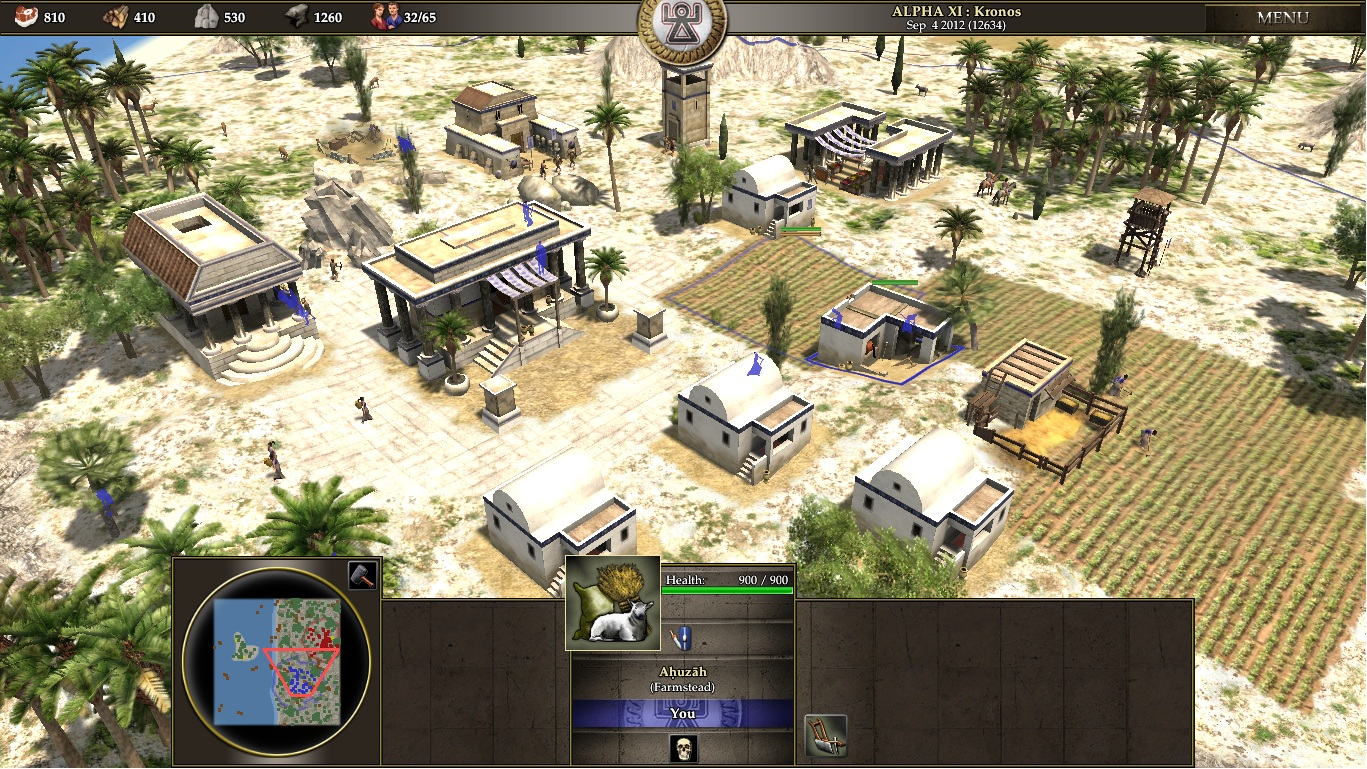
\includegraphics[width=0.9\textwidth]{ch2/0ad}
    \caption{Typical in-game view of 0 A.D., an open source cross-platform
      Real-Time Strategy game.}
    \label{fig:0ad}
\end{figure}

Real-Time strategy (RTS) games have historically been a source of complex
problems for AI researchers. The domain they usually construct is essentially a
simplified military simulation where players fight in a fixed-size 2D map for
the control of the finite amount of available resources. The players then have
to build armies and maintain a strong economy for them to win battles and,
ultimately, the overall game. The variety of AI and decision-making problems
that this typology of games requires solving include (but are not limited to):

\begin{itemize}
  \item Decision making under uncertainty.
  \item Opponent modelling and Learning.
  \item Resource management.
  \item Real-time planning.
  \item Exploration/exploitation dilemma.
\end{itemize}

Those are all terribly challenging problems that have spawned several techniques
and even entire areas of research \citep{buro2003real}. The creation of a
machine learning system that can at least partially solve all those problems and
therefore have the chance to have a fair game against a human opponent is far
from being close, even with the relatively game-changing performances of Deep
Reinforcement Learning.

Over the years several RTS research platforms have in the AI community:

\begin{description}
\item [Stratagus \citep{ponsen2005stratagus}] - Open-source and cross-platform,
  Stratagus is a platform that allows to build Blizzard's Warcraft-like RTS
  games. To upgrade it to a AI research platform in 2005 researchers connect
  TIELT, the Testbed for Integrating and Evaluating Learning Techniques, to the
  game \citep{molineaux2005tielt}.
\item [ORTS \citep{buro2002orts}] - Planned from the start to be a RTS
  research platform, this game is a rough port of StarCraft: Brood War.
  Unfortunately most of the development seems to have stopped around 2010.
\item [FreeCiv \citep{houk2004strategic}] - Open-source game used for research
  on Civilisation-like strategy games. While not quite a real-time strategy
  game, the domain forces players to focus both on micro-management and strategy
  planning in a similar fashion.
\end{description} 

While those (and other) games exploit the flexibility of their open-source
solutions making them often completely modifiable to suit for a large set of
needs, most of them lack polish in terms of game-mechanics and general software
robustness to be used as AI platforms. Commercial games have instead a better
support on most ecosystems and allow researchers to take advantage of the
players community to collect useful data. This is a critical advantage given how
data-hungry most of the current state-of-the-art machine learning systems have
become. A more feasible solution is therefore to take one of the popular
commercial games and adapt it to create an AI testing suite.

\subsection{StarCraft Brood War}

StarCraft is a relatively old commercial game developed in 1998 by Blizzard
Entertainment, Inc. that represents the quintessence of Real-Time Strategy
games. Since the beginning it has attracted tens of millions of players, selling
as many copies and pioneering the use of video games as competitive e-sport
platforms. As a consequence StarCraft has been used as a platform for
professional competitions for nearly 20 years, generating annually an industry
of several millions of US dollars. When StarCraft 2 was released in 2009, the
game sold even more copies, creating another wave of excitement towards online
gaming that has yet to stop growing. The popularity of this game gives us a
great motivation to work towards providing the artificial intelligence and
machine learning communities a way to control the game and use the massive
amount of collected playing data available online to seriously start tackling
the complexity of Real-Time Strategy games.

\begin{figure}[h]
    \centering
    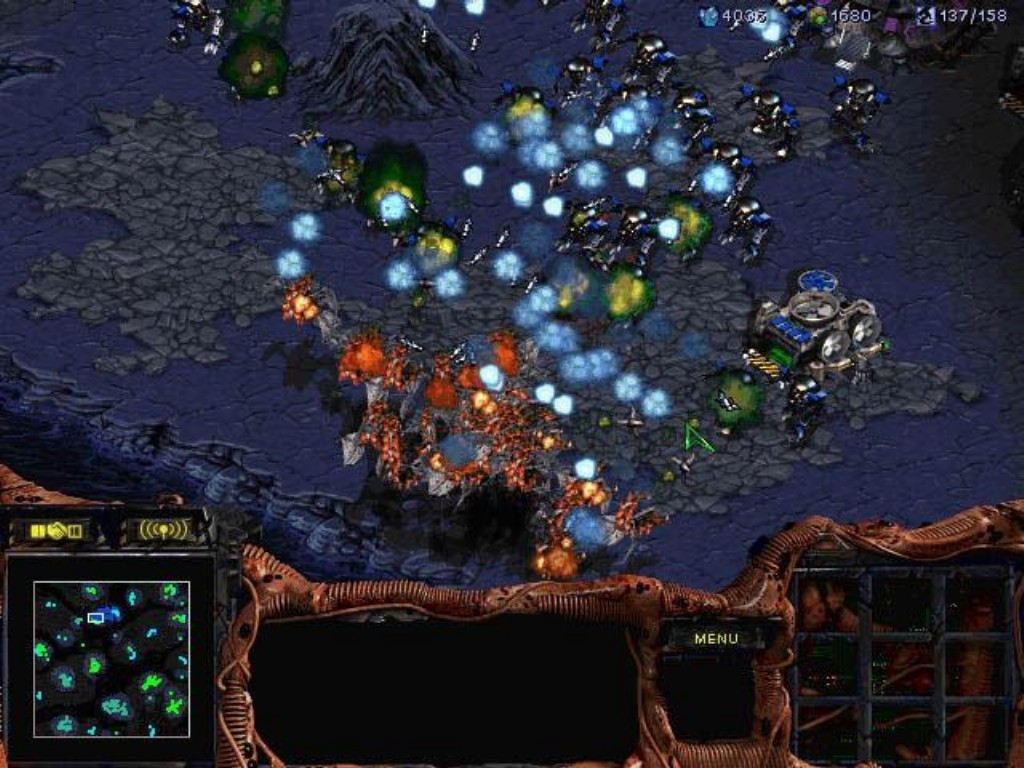
\includegraphics[width=0.9\textwidth]{ch2/scbw_temp}
    \caption{Typical in-game screen of a StarCraft Brood War match.}
    \label{fig:ALE}
\end{figure}

\section{Previous work on RTS games}

Real-Time Strategy games decision-making can be categorised into three main
sub-problems based on military literature (in descending level of abstraction):
\emph{strategy}, \emph{tactics} and \emph{reactive} behaviour
\citep{handel2005masters}. The higher the abstraction, the more likely
decision-making tends to take the form of strategical behaviour, the more local
the more likely the process will need to be more reactive and related to
single-unit control.

Most of previous work in RTS games has been constructed around the idea of using
pre-engineered knowledge and solving only parts of the entire problem. Several
aspects of the game have been studied:

\begin{description}
\item [Opponent modelling] - as players start with no vision of their opponent
  units or actions, the initial part of the game consists in quickly exploring
  the environment and understand the overall strategy of the opponent. As the
  game carries on, more complex strategy prediction needs to be done to
  successfully win the game (very similarly to games like rock-paper-scissors). 
  Examples of previous work focused on modelling opponent behaviour are
  \cite{dereszynski2011learning, schadd2007opponent, synnaeve2012special}.
\item [Strategy selection] - given a pool of parametrisable strategies, machine
  learning can be used to optimise the decision-making process at each point of
  the hierarchy. Examples of such work are \cite{ontanon2008learning,
    weber2010reactive, young2012evolutionary}.
\item [Build-order planning] - a lot of RTS decision-making focuses on balancing
  exploitation of the environment and continuous exploration. Acquiring control
  of the resources is a primary goal of the game, and this is often done by
  optimising the process of building army and structures compositions. Examples
  of previous work are \cite{churchill2011build, kovarsky2006first,
    weber2009case}.
\item [Combat timing and optimisation] - RTS games are usually well-balanced and
  strategies require employing the correct units and micromanaging attacks.
  Nearly all the literature on reactive planning applies in this case, but
  examples of relevant work done in micro-management of RTS games' units are
  \cite{balla2009uct, certicky2013case, kovarsky2005heuristic}. 
\end{description}

Many more papers are available on the subject, with other subproblems being
relevant to StarCraft and other Real-Time Strategy games. A broader discussion
is available at \cite{ontanon2013survey} and \cite{churchill2016heuristic}.

\subsubsection{RTS AI Competitions}

The first RTS research competition was created by a group at the University of
Alberta in 2006 with the goal of creating agents to play Open RTS
\citep{buro2002orts}. This first competition focused on separately solving some
aspects of the game such as small combat scenarios and scalable resource
gathering. 

The first StarCraft AI competition was organized by a group at the University of
California, Santa Cruz during AIIDE, a popular game AI conference. Following
years saw a constant increase in participation and two additional StarCraft AI
competitions being created: CIG and SSCAI \citep{buro2012real}. Those
competitions led AI researchers and programmers to focus on the entire game and
to adapt their algorithms to work in the same conditions that human players
usually have to deal with. This was done with the goal to eventually take on
professional gamers in the same way AI research had previously tried to beat
professional board games players.

\section{Summary}

The first part of this chapter has presented the Reinforcement Learning
framework and the Markov Decision Process, a formalisation of decision-making
tasks that allows to study, analyse and compare reinforcement learning
algorithms. In particular we have looked at research focused on adding some form
of hierarchical structure to reinforcement learning as a way to address the
problem of learning growing policy spaces. Additionally we have looked at recent
work that addresses the problem of learning policies from visual information
using deep learning, a powerful set of algorithms for building generative models
that can automatically discover features and that work surprisingly well for
domains when lots of data is available.

The second part of the chapter has focused on reviewing some of the available
video-game platforms that have successfully been used in artificial intelligence
research, looking in particular at Real-Time Strategy games. Finally we have
provided a description of StarCraft, its properties and the rationale behind the
idea of transforming it into a fully-fledged agent learning platform.